\documentclass[onlymath]{beamer}
% \documentclass[onlymath,handout]{beamer}

% Macros used by all lectures, but not necessarily by excercises

%%% General setup and dependencies:

% \usetheme[ddcfooter,nosectionnum]{tud}
\usetheme[nosectionnum,pagenum,noheader]{tud}
% \usetheme[nosectionnum,pagenum]{tud}

% Increase body font size to a sane level:
\let\origframetitle\frametitle
% \renewcommand{\frametitle}[1]{\origframetitle{#1}\normalsize}
\renewcommand{\frametitle}[1]{\origframetitle{#1}\fontsize{10pt}{13.2}\selectfont}
\setbeamerfont{itemize/enumerate subbody}{size=\small} % tud defaults to scriptsize!
\setbeamerfont{itemize/enumerate subsubbody}{size=\small}
% \setbeamerfont{normal text}{size=\small}
% \setbeamerfont{itemize body}{size=\small}

\renewcommand{\emph}[1]{\textbf{#1}}

\def\arraystretch{1.3}% Make tables even less cramped vertically

\usepackage[ngerman]{babel}
\usepackage[utf8]{inputenc}
\usepackage[T1]{fontenc}

%\usepackage{graphicx}
\usepackage[export]{adjustbox} % loads graphicx
\usepackage{import}
\usepackage{stmaryrd}
\usepackage[normalem]{ulem} % sout command
% \usepackage{times}
\usepackage{txfonts}

% \usepackage[perpage]{footmisc} % reset footnote counter on each page -- fails with beamer (footnotes gone)
\usepackage{perpage}  % reset footnote counter on each page
\MakePerPage{footnote}

\usepackage{tikz}
\usetikzlibrary{arrows,positioning}
% Inspired by http://www.texample.net/tikz/examples/hand-drawn-lines/
\usetikzlibrary{decorations.pathmorphing}
\pgfdeclaredecoration{penciline}{initial}{
    \state{initial}[width=+\pgfdecoratedinputsegmentremainingdistance,
    auto corner on length=1mm,]{
        \pgfpathcurveto%
        {% From
            \pgfqpoint{\pgfdecoratedinputsegmentremainingdistance}
                      {\pgfdecorationsegmentamplitude}
        }
        {%  Control 1
        \pgfmathrand
        \pgfpointadd{\pgfqpoint{\pgfdecoratedinputsegmentremainingdistance}{0pt}}
                    {\pgfqpoint{-\pgfdecorationsegmentaspect
                     \pgfdecoratedinputsegmentremainingdistance}%
                               {\pgfmathresult\pgfdecorationsegmentamplitude}
                    }
        }
        {%TO 
        \pgfpointadd{\pgfpointdecoratedinputsegmentlast}{\pgfpoint{1pt}{1pt}}
        }
    }
    \state{final}{}
}
\tikzset{handdrawn/.style={decorate,decoration=penciline}}
\tikzset{every shadow/.style={fill=none,shadow xshift=0pt,shadow yshift=0pt}}
% \tikzset{module/.append style={top color=\col,bottom color=\col}}

% Use to make Tikz attributes with Beamer overlays
% http://tex.stackexchange.com/a/6155
\tikzset{onslide/.code args={<#1>#2}{%
  \only<#1| handout:0>{\pgfkeysalso{#2}} 
}}
\tikzset{onslideprint/.code args={<#1>#2}{%
  \only<#1>{\pgfkeysalso{#2}} 
}}

%%% Title -- always set this first

\newcommand{\defineTitle}[3]{
	\newcommand{\lectureindex}{#1}
	\title{Formale Systeme}
	\subtitle{\href{\lectureurl}{#1. Vorlesung: #2}}
	\author{\href{http://korrekt.org/}{Markus Kr\"{o}tzsch}}
%	\author{\href{http://www.sebastian-rudolph.de}{Sebastian Rudolph} in Vertretung von \href{http://korrekt.org/}{Markus Kr\"{o}tzsch}}
	\date{#3}
	\datecity{TU Dresden}
% 	\institute{Computational Logic}
}

%%% Table of contents:

\RequirePackage{ifthen}

\newcommand{\highlight}[2]{%
	\ifthenelse{\equal{#1}{\lectureindex}}{\alert{#2}}{#2}%
}

\def\myspace{-0.7ex}
\newcommand{\printtoc}{
\begin{tabular}{r@{$\quad$}l}
\highlight{1}{1.} & \highlight{1}{Willkommen/Einleitung formale Sprachen}\\[\myspace]
\highlight{2}{2.} & \highlight{2}{Grammatiken und die Chomsky-Hierarchie}\\[\myspace]
\highlight{3}{3.} & \highlight{3}{Endliche Automaten}\\[\myspace]
\highlight{4}{4.} & \highlight{4}{Complexity of FO query answering}\\[\myspace]
\highlight{5}{5.} & \highlight{5}{Conjunctive queries}\\[\myspace]
\highlight{6}{6.} & \highlight{6}{Tree-like conjunctive queries}\\[\myspace]
\highlight{7}{7.} & \highlight{7}{Query optimisation}\\[\myspace]
\highlight{8}{8.} & \highlight{8}{Conjunctive Query Optimisation / First-Order~Expressiveness}\\[\myspace]
\highlight{9}{9.} & \highlight{9}{First-Order~Expressiveness / Introduction to Datalog}\\[\myspace]
\highlight{10}{10.} & \highlight{10}{Expressive Power and Complexity of Datalog}\\[\myspace]
\highlight{11}{11.} & \highlight{11}{Optimisation and Evaluation of Datalog}\\[\myspace]
\highlight{12}{12.} & \highlight{12}{Evaluation of Datalog (2)}\\[\myspace]
\highlight{13}{13.} & \highlight{13}{Graph Databases and Path Queries}\\[\myspace]
\highlight{14}{14.} & \highlight{14}{Outlook: database theory in practice}
\end{tabular}
}

\newcommand{\overviewslide}{%
\begin{frame}\frametitle{Overview}
\printtoc
\medskip

Siehe \href{\lectureurl}{course homepage [$\Rightarrow$ link]} for more information and materials
\end{frame}
}

%%% Colours:

\usepackage{xcolor,colortbl}
\definecolor{redhighlights}{HTML}{FFAA66}
\definecolor{lightblue}{HTML}{55AAFF}
\definecolor{lightred}{HTML}{FF5522}
\definecolor{lightpurple}{HTML}{DD77BB}
\definecolor{lightgreen}{HTML}{55FF55}
\definecolor{darkred}{HTML}{CC4411}
\definecolor{darkblue}{HTML}{176FC0}%{1133AA}
\definecolor{nightblue}{HTML}{2010A0}%{1133AA}
\definecolor{alert}{HTML}{176FC0}
\definecolor{darkgreen}{HTML}{36AB14}
\definecolor{strongyellow}{HTML}{FFE219}
\definecolor{devilscss}{HTML}{666666}

\newcommand{\redalert}[1]{\textcolor{darkred}{#1}}

%%% Style commands

\newcommand{\quoted}[1]{\texttt{"}{#1}\texttt{"}}
\newcommand{\squote}{\texttt{"}} % straight quote
\newcommand{\Sterm}[1]{\ensuremath{\mathtt{\textcolor{purple}{#1}}}}    % letters in alphabets
\newcommand{\Snterm}[1]{\textsf{\textcolor{darkblue}{#1}}} % nonterminal symbols
\newcommand{\Sntermsub}[2]{\Snterm{#1}_{\Snterm{#2}}} % nonterminal symbols
\newcommand{\Slang}[1]{\textbf{\textcolor{black}{#1}}}    % languages
\newcommand{\Slangsub}[2]{\Slang{#1}_{\Slang{#2}}}    % languages
% Code
\newcommand{\Scode}[1]{\textbf{#1}}    % reserved words in program listings, e.g., "if"
\newcommand{\Scodelit}[1]{\textcolor{purple}{#1}}    % literals in program listings, e.g., strings
\newcommand{\Scomment}[1]{\textcolor{gray}{#1}}    % comment in program listings

\newcommand{\epstrastar}{\mathrel{\mathord{\stackrel{\epsilon}{\to}}{}^*}} % transitive reflexive closure of epsilon transitions in an epslion-NFA

\newcommand{\narrowcentering}[1]{\mbox{}\hfill#1\hfill\mbox{}}

\newcommand{\defeq}{\mathrel{:=}}

\newcommand{\Smach}[1]{\ensuremath{\mathcal{#1}}}    % machines

%%% Slide layout commands:

\newcommand{\sectionSlide}[1]{
\frame{\begin{center}
\LARGE
#1
\end{center}}
}
\newcommand{\sectionSlideNoHandout}[1]{
\frame<handout:0>{\begin{center}
\LARGE
#1
\end{center}}
}

\newcommand{\mydualbox}[3]{%
 \begin{minipage}[t]{#1}
 \begin{beamerboxesrounded}[upper=block title,lower=block body,shadow=true]%
    {\centering\usebeamerfont*{block title}#2}%
    \raggedright%
    \usebeamerfont{block body}
%     \small
    #3%
  \end{beamerboxesrounded}
  \end{minipage}
}
% 
\newcommand{\myheaderbox}[2]{%
 \begin{minipage}[t]{#1}
 \begin{beamerboxesrounded}[upper=block title,lower=block title,shadow=true]%
    {\centering\usebeamerfont*{block title}\rule{0pt}{2.6ex} #2}%
  \end{beamerboxesrounded}
  \end{minipage}
}

\newcommand{\mycontentbox}[2]{%
 \begin{minipage}[t]{#1}%
 \begin{beamerboxesrounded}[upper=block body,lower=block body,shadow=true]%
    {\centering\usebeamerfont*{block body}\rule{0pt}{2.6ex}#2}%
  \end{beamerboxesrounded}
  \end{minipage}
}

\newcommand{\mylcontentbox}[2]{%
 \begin{minipage}[t]{#1}%
 \begin{beamerboxesrounded}[upper=block body,lower=block body,shadow=true]%
    {\flushleft\usebeamerfont*{block body}\rule{0pt}{2.6ex}#2}%
  \end{beamerboxesrounded}
  \end{minipage}
}

% label=180:{\rotatebox{90}{{\footnotesize\textcolor{darkgreen}{Beispiel}}}}
% \hspace{-8mm}\ghost{\raisebox{-7mm}{\rotatebox{90}{{\footnotesize\textcolor{darkgreen}{Beispiel}}}}}\hspace{8mm}
\newcommand{\examplebox}[1]{%
	\begin{tikzpicture}[decoration=penciline, decorate]
		\pgfmathsetseed{1235}
		\node (n1) [decorate,draw=darkgreen, fill=darkgreen!10,thick,align=left,text width=\linewidth, inner ysep=2mm, inner xsep=2mm] at (0,0) {#1};
% 		\node (n2) [align=left,text width=\linewidth,inner sep=0mm] at (n1.92) {{\footnotesize\raisebox{3mm}{\textcolor{darkgreen}{Beispiel}}}};
% 		\node (n2) [decorate,draw=darkgreen, fill=darkgreen!10,thick, align=left,text width=\linewidth,inner sep=2mm] at (n1.90) {{\footnotesize\raisebox{0mm}{\textcolor{darkgreen}{Beispiel}}}};
	\end{tikzpicture}%
}%

\newcommand{\codebox}[1]{%
	\begin{tikzpicture}[decoration=penciline, decorate]
		\pgfmathsetseed{1236}
		\node (n1) [decorate,draw=strongyellow, fill=strongyellow!10,thick,align=left,text width=\linewidth, inner ysep=2mm, inner xsep=2mm] at (0,0) {#1};
	\end{tikzpicture}%
}%

\newcommand{\defbox}[1]{%
	\begin{tikzpicture}[decoration=penciline, decorate]
		\pgfmathsetseed{1237}
		\node (n1) [decorate,draw=darkred, fill=darkred!10,thick,align=left,text width=\linewidth, inner ysep=2mm, inner xsep=2mm] at (0,0) {#1};
	\end{tikzpicture}%
}%

\newcommand{\theobox}[1]{%
	\begin{tikzpicture}[decoration=penciline, decorate]
		\pgfmathsetseed{1240}
		\node (n1) [decorate,draw=darkblue, fill=darkblue!10,thick,align=left,text width=\linewidth, inner ysep=2mm, inner xsep=2mm] at (0,0) {#1};
	\end{tikzpicture}%
}%

\newcommand{\anybox}[2]{%
	\begin{tikzpicture}[decoration=penciline, decorate]
		\pgfmathsetseed{1240}
		\node (n1) [decorate,draw=#1, fill=#1!10,thick,align=left,text width=\linewidth, inner ysep=2mm, inner xsep=2mm] at (0,0) {#2};
	\end{tikzpicture}%
}%


\newsavebox{\mybox}%
\newcommand{\doodlebox}[2]{%
\sbox{\mybox}{#2}%
	\begin{tikzpicture}[decoration=penciline, decorate]
		\pgfmathsetseed{1238}
		\node (n1) [decorate,draw=#1, fill=#1!10,thick,align=left,inner sep=1mm] at (0,0) {\usebox{\mybox}};
	\end{tikzpicture}%
}%

% Common notation

\usepackage{amsmath,amssymb,amsfonts}
\usepackage{xspace}

\newcommand{\lectureurl}{https://iccl.inf.tu-dresden.de/web/FS2016}

\DeclareMathAlphabet{\mathsc}{OT1}{cmr}{m}{sc} % Let's have \mathsc since the slide style has no working \textsc

% Dual of "phantom": make a text that is visible but intangible
\newcommand{\ghost}[1]{\raisebox{0pt}[0pt][0pt]{\makebox[0pt][l]{#1}}}

\newcommand{\tuple}[1]{\langle{#1}\rangle}

%%% Annotation %%%

\usepackage{color}
\newcommand{\todo}[1]{{\tiny\color{red}\textbf{TODO: #1}}}



%%% Old macros below; move when needed

\newcommand{\blank}{\text{\textvisiblespace}} % empty tape cell for TM

% table syntax
\newcommand{\dom}{\textbf{dom}}
\newcommand{\adom}{\textbf{adom}}
\newcommand{\dbconst}[1]{\texttt{"#1"}}
\newcommand{\pred}[1]{\textsf{#1}}
\newcommand{\foquery}[2]{#2[#1]}
\newcommand{\ground}[1]{\textsf{ground}(#1)}
% \newcommand{\foquery}[2]{\{#1\mid #2\}} %% Notation as used in Alice Book
% \newcommand{\foquery}[2]{\tuple{#1\mid #2}}

\newcommand{\quantor}{\mathord{\reflectbox{$\text{\sf{Q}}$}}} % the generic quantor

% logic syntax
\newcommand{\Inter}{\mathcal{I}} %used to denote an interpretation
\newcommand{\Jnter}{\mathcal{J}} %used to denote another interpretation
\newcommand{\Knter}{\mathcal{K}} %used to denote yet another interpretation
\newcommand{\Zuweisung}{\mathcal{Z}} %used to denote a variable assignment

% query languages
\newcommand{\qlang}[1]{{\sf #1}} % Font for query languages
\newcommand{\qmaps}[1]{\textbf{QM}({\sf #1})} % Set of query mappings for a query language

%%% Complexities %%%

\hyphenation{Exp-Time} % prevent "Ex-PTime" (see, e.g. Tobies'01, Glimm'07 ;-)
\hyphenation{NExp-Time} % better that than something else

% \newcommand{\complclass}[1]{{\sc #1}\xspace} % font for complexity classes
\newcommand{\complclass}[1]{\ensuremath{\mathsc{#1}}\xspace} % font for complexity classes

\newcommand{\ACzero}{\complclass{AC$_0$}}
\newcommand{\LogSpace}{\complclass{L}}
\newcommand{\NLogSpace}{\complclass{NL}}
\newcommand{\PTime}{\complclass{P}}
\newcommand{\NP}{\complclass{NP}}
\newcommand{\coNP}{\complclass{coNP}}
\newcommand{\PH}{\complclass{PH}}
\newcommand{\PSpace}{\complclass{PSpace}}
\newcommand{\NPSpace}{\complclass{NPSpace}}
\newcommand{\ExpTime}{\complclass{ExpTime}}
\newcommand{\NExpTime}{\complclass{NExpTime}}
\newcommand{\ExpSpace}{\complclass{ExpSpace}}
\newcommand{\TwoExpTime}{\complclass{2ExpTime}}
\newcommand{\NTwoExpTime}{\complclass{N2ExpTime}}
\newcommand{\ThreeExpTime}{\complclass{3ExpTime}}
\newcommand{\kExpTime}[1]{\complclass{#1ExpTime}}
\newcommand{\kExpSpace}[1]{\complclass{#1ExpSpace}}

% 
% Der folgende Algorithmus erzeugt die im ersten Fall gesuchte Formel:
% \begin{itemize}
% \item Solange es eine Teilformel $G\leftrightarrow H$ in $F$ gibt, ersetze $G\leftrightarrow H$ durch $\neg (G\wedge\neg H)\wedge\neg (H\wedge\neg G)$
% \item Solange es eine Teilformel $G\to H$ in $F$ gibt, ersetze $G\to H$ durch $\neg (G\wedge\neg H)$
% \item Solange es eine Teilformel $G\vee H$ in $F$ gibt, ersetze $G\vee H$ durch $\neg(\neg G\wedge\neg H)$
% \end{itemize}
% Dieser

\usepackage{setspace}

\defineTitle{22}{Äquivalenzen und Normalformen}{12. Januar 2017}

\begin{document}

\maketitle

\sectionSlideNoHandout{Rückblick}

\begin{frame}\frametitle{Aussagenlogik}

\emph{Syntax:}
\[ \Snterm{F}\to \Slang{P}\mid \Sterm{\neg}\Snterm{F}\mid\Sterm{(}\Snterm{F}\Sterm{\wedge}\Snterm{F}\Sterm{)} \mid\Sterm{(}\Snterm{F}\Sterm{\vee}\Snterm{F}\Sterm{)} \mid\Sterm{(}\Snterm{F}\Sterm{\to}\Snterm{F}\Sterm{)} \mid\Sterm{(}\Snterm{F}\Sterm{\leftrightarrow}\Snterm{F}\Sterm{)}
\]

\emph{Semantik:}
\begin{itemize}
\item Wertzuweisungen $w:\Slang{P}\to\{\mytrue,\myfalse\}$ zur Interpretation von Atomen
\item Erweiterung von Atomen auf Formeln:
\footnotesize
\narrowcentering{%
\begin{tabular}[t]{cc}
\rowcolor{lightblue!20}
$w(F)$ & $w(\neg F)$\\
\myfalse & \mytrue \\
\rowcolor{gray!10}
\mytrue & \myfalse \\
\end{tabular}}\medskip

\begin{tabular}{cccccc}
\rowcolor{lightblue!20}
$w(F)$ & $w(G)$ & $w(F\wedge G)$ & $w(F\vee G)$ & $w(F\to G)$ & $w(F\leftrightarrow G)$\\
\myfalse & \myfalse & \myfalse & \myfalse& \mytrue & \mytrue\\
\rowcolor{gray!10}
\mytrue & \myfalse & \myfalse & \mytrue& \myfalse & \myfalse\\
\myfalse & \mytrue & \myfalse & \mytrue& \mytrue & \myfalse\\
\rowcolor{gray!10}
\mytrue & \mytrue & \mytrue & \mytrue& \mytrue & \mytrue\\
\end{tabular}

\end{itemize}

\end{frame}


\begin{frame}\frametitle{Logische Schlussfolgerung}

\emph{Modelle:}\smallskip

$w\models F$ \alert{gdw.} $w(F)=\mytrue$ \alert{gdw.} "`$w$ ist Modell von $F$"' \alert{gdw.} "`$w$ erfüllt $F$"'
\bigskip

\emph{Logische Konsequenzen:}
\begin{itemize}
\item $\mathcal{F}\models G$ \alert{gdw.}
\item jedes Modell von $\mathcal{F}$ ist auch ein Modell von $G$ \alert{gdw.}
\item $G$ ist immer wahr wenn alle Formeln in $\mathcal{F}$ wahr sind
\end{itemize}\pause

\emph{Dualität von Modellen und Formeln:}
\begin{itemize}
\item Je mehr Formeln in $\mathcal{F}$
\item desto weniger Modelle erfüllen alle Formeln in $\mathcal{F}$
\item desto mehr Formeln sind in allen diesen Modellen wahr
\item desto mehr Konsequenzen hat $\mathcal{F}$
\end{itemize}
$\leadsto$ Aussagenlogik ist \redalert{monoton} (mehr Annahmen $\Rightarrow$ mehr Schlüsse)

\end{frame}

\begin{frame}\frametitle{Modellierungsbeispiel: Sudoku (1)}

Sudoku ist ein bekanntes Zahlenpuzzle.
\bigskip

\narrowcentering{
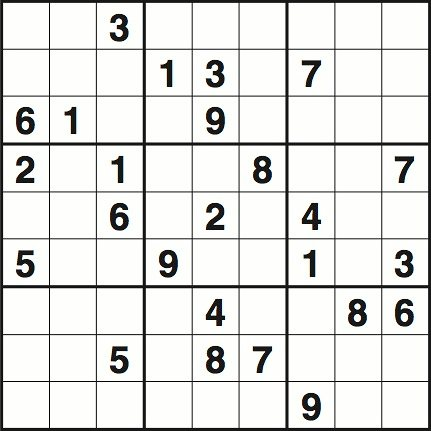
\includegraphics[height=4cm]{images/Sudoku}
}

Aufgabe: 
\begin{itemize}
\item Fülle jedes Feld mit einer Ziffer von $1$ bis $9$, so dass
\item Spalten, Zeilen und die fetten Teilquadrate jede Ziffer nur einmal enthalten
\end{itemize}

\end{frame}

\begin{frame}\frametitle{Modellierungsbeispiel: Sudoku (2)}

Wir können Sudoku aussagenlogisch modellieren:\pause

\begin{itemize}
\item \alert{Atome:} Für jede Ziffer $z\in\{1,\ldots,9\}$ und alle Koordinaten $i,j\in\{1,\ldots,9\}$ verwenden wir ein Atom $p_z[i,j]$ für die Aussage "`an Position $(i,j)$ steht die Ziffer $z$"'
\pause
\item \alert{Spielregeln} modellieren wir als logische Formeln:
\end{itemize}\vspace{-2.5ex}
\begin{align*}
\text{Für alle $i,j$:} & \quad p_1[i,j]\vee p_2[i,j]\vee\ldots\vee p_9[i,j] %& \quad\text{(mindestens eine Ziffer pro Feld)}
\\
\text{Für alle $i,j,z,z'$ mit $z\neq z'$:} & \quad p_z[i,j] \to \neg p_{z'}[i,j] %& \text{(höchstens eine Ziffer pro Feld)}
\\
\text{Für alle $i,i',j,z$ mit $i\neq i'$:} & \quad p_z[i,j] \to \neg p_z[i',j] %& \text{(höchstens eine Ziffer pro Feld)}
\\
\text{Für alle $i,j,j',z$ mit $j\neq j'$:} & \quad p_z[i,j] \to \neg p_z[i,j'] %& \text{(höchstens eine Ziffer pro Feld)}
\\
\text{Für alle $i,j,i',j',z$ mit $(i,j)\neq (i',j')$;}\\
\text{$(i,j)$, $(i',j')$  im gleichen Teilquadrat:} & \quad p_z[i,j] \to \neg p_z[i',j'] %& \text{(höchstens eine Ziffer pro Feld)}
\end{align*}\vspace{-4ex}\pause
\begin{itemize}
\item \alert{Vorgegebene Ziffern} werden als atomare Formeln dargestellt, z.B. $p_3[3,1]$ im vorigen Beispiel
\end{itemize}\pause
$\leadsto$ Modelle der Formelmenge entsprechen Lösungen des Sudoku

\end{frame}


\sectionSlide{Äquivalenzen}

\newcommand{\emphcell}[1]{\only<#1>{\cellcolor{strongyellow}}}

\begin{frame}\frametitle{Logische Äquivalenz}

Formeln sind äquivalent, wenn sie die gleiche Semantik haben:

\defbox{Zwei Formeln $F$ und $G$ sind \redalert{semantisch äquivalent}, in Symbolen \redalert{$F\equiv G$},
wenn sie genau die selben Modelle haben, d.h. wenn\\[1ex]

\narrowcentering{für alle Wertzuweisungen $w$ gilt: $w(F)=w(G)$}}\pause

\examplebox{Beispiel: $p\to q \equiv \neg p\vee q$, wie man mithilfe der Wahrheitswertetabelle zeigen kann (die Spalten der Formeln sind gleich):\smallskip

\narrowcentering{%
\begin{tabular}{cccccc}
\rowcolor{darkgreen!30}
$p$ & $q$ & $p\to q$ & $\neg p$ & $\neg p\vee q$ & ${}^*$\\
\myfalse & \myfalse & \emphcell{3-}{\mytrue} & \mytrue & \emphcell{3-}{\mytrue} \\
\mytrue & \myfalse & \emphcell{3-}{\myfalse} & \myfalse & \emphcell{3-}{\myfalse} \\
\myfalse & \mytrue & \emphcell{3-}{\mytrue} & \mytrue & \emphcell{3-}{\mytrue} \\
\mytrue & \mytrue & \emphcell{3-}{\mytrue} & \myfalse & \emphcell{3-}{\mytrue} \\
\end{tabular}}
}

{\footnotesize ${}^*$ Vereinfachung: Wir beschriften Tabellenspalten ab jetzt nur mit $F$ statt \ghost{$w(F)$.}}

\end{frame}

\begin{frame}\frametitle{Nützliche Eigenschaften von $\equiv$}

\theobox{Satz: $\equiv$ ist eine Äquivalenzrelation, d.h. reflexiv, symmetrisch und transitiv.}

\emph{Beweis:} $\equiv$ ist definiert als die Gleichheit der Modellmengen. Die gesuchten Eigenschaften ergeben sich, da auch die Relation $=$ auf Mengen eine Äquivalenzrelation ist.\qed
\bigskip

Weitere Eigenschaften folgen direkt aus den Definitionen:\medskip

\theobox{Satz:
\begin{itemize}
\item Alle Tautologien sind semantisch äquivalent
\item Alle unerfüllbaren Formeln sind semantisch äquivalent
\end{itemize}
}

% \emph{Beweis:} Offensichtlich sind die Modellmengen jeweils gleich.\qed

\theobox{Satz: Semantische Äquivalenz entspricht wechselseitiger logischer Konsequenz:\\[1ex]
% 
\narrowcentering{ $F\equiv G$ \hspace{5mm}genau dann wenn\hspace{5mm} $F\models G$ und $G\models F$}
}

\end{frame}

\begin{frame}\frametitle{Nützliche Eigenschaften von $\equiv$}

% 
% \emph{Intuition:} Äquivalente Formeln sind untereinander austauschbar, da sie sich logisch immer gleich verhalten
% \bigskip


\theobox{Satz (Ersetzungstheorem): Sei $F$ eine Formel mit einer Teilformel $G$. 
Wenn $G\equiv G'$ und wenn $F'$ aus $F$ gebildet werden kann, indem man ein beliebiges Vorkommen von $G$ in $F$ durch $G'$ ersetzt, dann gilt auch $F\equiv F'$.}\pause

\emph{Beweisskizze${}^*$:} Aus $G\equiv G'$ bedeutet, dass $w\models G$ gdw. $w\models G'$ für beliebige Wertzuweisungen $w$.
% Gemäß der rekursiven Definition von $\models$ hängt $w\models H$ nur davon ab, welche der direkten Unterformeln von
% $H$ durch $w$ erfüllt sind.
In der rekursiven Definition von $\models$ erfüllt daher die Teilformel $G$ genau die selben Bedingungen wie $G'$, so
dass sich auch für $F$ und $F'$ der selbe Wert ergibt.\qed
\bigskip

Dieser Satz ist ein Sonderfall der allgemeingültigen und intuitiven Tatsache, dass der Wert von rekursiv definierten Funktionen gleich bleibt, wenn man die syntaktische Definition einer Teilberechnung durch eine andere ersetzt, die stets den gleichen Wert liefert.
\bigskip

\setstretch{0.9}

{\tiny ${}^*$ Streng genommen folgt aus der Definition von $\models$ zunächst nur, dass die Ersetzung einer direkten Unterformel
Äquivalenz erhält. Zum Beispiel folgt $G\wedge H\equiv G'\wedge H$ aus $G\equiv G'$. Um zu zeigen, dass auch Ersetzungen in beliebiger Tiefe Äquivalenz erhalten, ist noch ein induktives Argument nötig, welches die Äquivalenz im Formelbaum "`nach oben"' propagiert. Aus $G\wedge H\equiv G'\wedge H$ folgt z.B. $(G\wedge H)\vee J\equiv (G'\equiv H)\vee J$ usw. usf.
}

\end{frame}

\begin{frame}\frametitle{Junktoren äquivalent ausdrücken}

Viele Junktoren können durch andere ausgedrückt werden:
% 
\begin{align*}
F\to G & \equiv \neg F\vee G \equiv \neg(F\wedge\neg G) \\
F\leftrightarrow G & \equiv (F\to G)\wedge(G\to F)\equiv (F\wedge G)\vee(\neg F\wedge \neg G) \\
F\wedge G & \equiv \neg(\neg F\vee\neg G) \quad \text{\textcolor{devilscss}{(De Morgansches Gesetz)}} \\
F\vee G & \equiv \neg(\neg F\wedge\neg G) \quad \text{\textcolor{devilscss}{(De Morgansches Gesetz)}}
\end{align*}\pause
%
Weitere Junktoren können mithilfe äquivalenter Formeln definiert werden:
% 
\begin{align*}
F\uparrow G & \equiv \neg (F\wedge G) \equiv \neg F\vee \neg G & \text{\textcolor{devilscss}{(NAND)}}\\
F\downarrow G & \equiv \neg (F\vee G) \equiv \neg F\wedge \neg G & \text{\textcolor{devilscss}{(NOR)}}\\
\top & \equiv \neg p\vee p \equiv p\to p & \text{\textcolor{devilscss}{(Wahrheit; $p\in\Slang{P}$ beliebig)}} \\
\bot & \equiv \neg p\wedge p & \text{\textcolor{devilscss}{(Falschheit; $p\in\Slang{P}$ beliebig)}}
\end{align*}\vspace{-4ex}

Wir werden insbesondere $\top$ und $\bot$ manchmal verwenden.

\end{frame}

\begin{frame}\frametitle{Junktoren äquivalent ausdrücken (2)}

% Mit dem Ersetzungstheorem folgt nun leicht:\medskip

\theobox{Satz: Sei $F$ eine beliebige aussagenlogische Formel.
\begin{itemize}
\item Es gibt eine zu $F$ äquivalente Formel, die nur die Junktoren $\wedge$ und $\neg$ enthält.
\item Es gibt eine zu $F$ äquivalente Formel, die nur die Junktoren $\vee$ und $\neg$ enthält.
\end{itemize}}\pause

\emph{Beweis:} Für den ersten Fall ersetzen wir iterativ Teilformeln, die nicht die gewünschte Form haben, gemäß den folgenden Regeln:
\begin{align*}
(G\vee H) &\qquad\mapsto\qquad \neg(\neg G\wedge\neg H)\\
(G\to H) &\qquad\mapsto\qquad\neg (G\wedge\neg H)\\
(G\leftrightarrow H) &\qquad\mapsto\qquad (\neg (G\wedge\neg H)\wedge\neg (H\wedge\neg G))
\end{align*}
Jede Ersetzung führt zu einer äquivalenten Formel (Ersetzungstheorem), der Algorithmus terminiert (jeder Junktor wird höchstens einmal ersetzt) und das Ergebnis hat die gewünschte Form.
% 
Der zweite Fall ist analog.
\qed

\end{frame}

\begin{frame}\frametitle{Nützliche Äquivalenzen (1)}

\begin{align*}
\begin{split}
F\wedge G & \equiv G\wedge F\\
F\vee G & \equiv G\vee F
\end{split}
		& \text{\textcolor{devilscss}{Kommutativität}} \\[1ex]
%
\begin{split}
(F\wedge G)\wedge H & \equiv F\wedge (G\wedge H)\\
(F\vee G)\vee H & \equiv F\vee (G\vee H)
\end{split}
		& \text{\textcolor{devilscss}{Assoziativität}} \\[1ex]
%
\begin{split}
F\wedge (G\vee H) & \equiv (F\wedge G) \vee (F\wedge H)\\
F\vee (G\wedge H) & \equiv (F\vee G)\wedge (F\vee H)
\end{split}
		& \text{\textcolor{devilscss}{Distributivität}} \\[1ex]
%
\begin{split}
F\wedge F & \equiv F\\
F\vee F & \equiv F
\end{split}
		& \text{\textcolor{devilscss}{Idempotenz}} \\[1ex]
%
\begin{split}
F\wedge (F\vee G) & \equiv F\\
F\vee (F\wedge G) & \equiv F
\end{split}
		& \text{\textcolor{devilscss}{Absorbtion}}
\end{align*}

\end{frame}

\begin{frame}\frametitle{Nützliche Äquivalenzen (2)}

\begin{align*}
\neg\neg F &\equiv F
		& \text{\textcolor{devilscss}{doppelte Negation}}\\[1ex]
%
\begin{split}
\neg(F\wedge G) & \equiv (\neg F\vee \neg G)\\
\neg(F\vee G) & \equiv (\neg F\wedge \neg G)
\end{split}
		& \text{\textcolor{devilscss}{De Morgansche Gesetze}} \\[1ex]
%
\begin{split}
F\wedge \top & \equiv F\\
F\vee \top & \equiv \top
\end{split}
		& \text{\textcolor{devilscss}{Gesetze mit $\top$}}\\[1ex]
%
\begin{split}
F\wedge \bot & \equiv \bot\\
F\vee \bot & \equiv F
\end{split}
		& \text{\textcolor{devilscss}{Gesetze mit $\bot$}}\\[1ex]
%
\begin{split}
\neg\top & \equiv \bot\\
\neg\bot & \equiv \top
\end{split}
		& 
\end{align*}

Alle diese Äquivalenzen können leicht mit Wahrheitswertetabellen überprüft werden.

\end{frame}

\begin{frame}\frametitle{Äquivalente Mengen von Formeln}

Die Definition von Äquivalenz ist leicht auf Formelmengen erweiterbar:\medskip

\defbox{Zwei Formelmengen $\mathcal{F}$ und $\mathcal{G}$ sind äquivalent, in Symbolen $\mathcal{F}\equiv\mathcal{G}$, wenn sie die selben Modelle haben.}\medskip\pause

Formelmengen verallgemeinern die Konjunktion, denn es gilt:\\[0.5ex]
%
\narrowcentering{
$ \{F_1,\ldots, F_n\}\equiv \{ F_1\wedge\ldots\wedge F_n\}$}\\[1ex]
%
\emph{Vereinfachung:} Dank Assoziativität verzichten wir ab jetzt in Formeln wie $(((F_1\wedge F_2)\wedge F_3)\wedge F_4)$
auf Klammern (ebenso für $\vee$).
\bigskip

Allerdings dürfen Formelmengen auch unendlich sein (Konjunktionen dagegen nicht).

\end{frame}

\begin{frame}\frametitle{$\models$ entspricht $\to$ und $\equiv$ entspricht $\leftrightarrow$}

\theobox{Satz (Deduktionstheorem): Für jede Formelmenge $\mathcal{F}$ und Formeln $G$ und $H$ gilt $\mathcal{F}\models G\to H$ genau dann wenn $\mathcal{F}\cup\{G\}\models H$.}\pause

\emph{Beweis:} Einfache Anwendung der Definitionen.
($\Rightarrow$) Wenn jedes Modell von $\mathcal{F}$ die Formel $G\to H$ erfüllt, 
dann muss jedes dieser Modelle, welches zudem $G$ erfüllt, $H$ erfüllen.  ($\Leftarrow$) Wenn jedes Modell von $\mathcal{F}$, welches zudem $G$ erfüllt, auch $H$ erfüllt, dann muss jedes Modell von $\mathcal{F}$ auch $G\to H$ erfüllen.\qed\medskip\pause

\anybox{purple}{Notation:
Wir schreiben $\models F$ statt $\emptyset\models F$ um auszudrücken, dass $F$ allgemeingültig ist.}

\theobox{Satz: $F\equiv G$ genau dann wenn $\models F\leftrightarrow G$.}\pause

\emph{Beweis:} $F\equiv G$ \alert{gdw.} $F\models G$ und $G\models F$ \alert{gdw.} $\models F\to G$ und $\models G\to F$ (wegen Deduktionstheorem) \alert{gdw.} $\models F\leftrightarrow G$. \qed

\end{frame}

\begin{frame}\frametitle{Curry}

Mit Deduktionstheorem und dem Bezug von Formelmengen und Konjunktionen erhält man ein weiteres interessantes
Ergebnis:\medskip

\narrowcentering{%
\begin{tabular}{@{}r@{~~}l@{~~}l@{}}
$\models (F\wedge G)\to H$ & gdw. $\{F\wedge G\}\models H$ & gdw. $\{F,G\}\models H$ \\
	& gdw. $\{F\}\models G\to H$ & gdw. $\models F\to (G\to H)$\\[1ex]
\end{tabular}}\medskip\pause

Tatsächlich gilt allgemein:
% 
\[ (F\wedge G)\to H\equiv F\to (G\to H)\]
% 
Die Ersetzung von $(F\wedge G)\to H$ durch $F\to (G\to H)$ wird \alert{Currying} (im Deutschen manchmal
auch: \alert{Schönfinkeln}) genannt\\
$\leadsto$ vgl. \redalert{funktionale Programmierung}

\end{frame}

\sectionSlideNoHandout{Normalformen}
% 
\begin{frame}\frametitle{}

~\hfill

\includegraphics[height=6.5cm]{images/aaron-swartz}~~
\rotatebox{90}{\tiny (C) Fred Benenson, 2008, CC-BY 2.0}
\hfill~

\narrowcentering{Aaron Swartz}\\
\narrowcentering{8. November 1986 -- 11. Januar 2013}\\
\narrowcentering{"`The Internet's Own Boy"'}


\end{frame}

\sectionSlide{Normalformen}

\begin{frame}\frametitle{Normalform}

\redalert{Normalformen} sind besondere syntaktische Formen aussagenlogischer Formeln
\bigskip

Sie heißen so, weil sich jede aussagenlogische Formel in eine äquivalente Formel in Normalform umformen lässt
\bigskip

Wir werden hier drei wichtige Normalformen kennenlernen:
\begin{itemize}
\item \alert{Negationsnormalform} (NNF)
\item \alert{Konjunktive Normalform} (KNF)
\item \alert{Disjunktive Normalform} (DNF)
\end{itemize}

\end{frame}

\begin{frame}\frametitle{Negationsnormalform}

\defbox{Eine Formel $F$ ist in \redalert{Negationsnormalform} (\alert{NNF}) wenn
\begin{enumerate}[(a)]
\item sie nur die Junktoren $\wedge$, $\vee$ und $\neg$ enthält und
\item der Junktor $\neg$ nur direkt vor Atomen vorkommt (d.h. nur in Teilformeln der Form $\neg p$ mit $p\in\Slang{P}$).
\end{enumerate}
}\medskip

Formeln, die negierte oder nicht-negierte Atome sind, nennt man \redalert{Literale}.
In NNF darf Negation also nur in Literalen auftauchen.
\medskip\pause

\examplebox{Beispiele:
\begin{itemize}
\item $(\neg p\wedge q)\vee (p\wedge\neg q)$ ist in NNF
\item $(b\wedge b)\vee\neg(b\wedge b)$ ist nicht in NNF
\item $q\vee \neg\neg p$ ist nicht in NNF
\item $p\leftrightarrow p$ ist nicht in NNF
\end{itemize}}

\end{frame}

\begin{frame}\frametitle{Umwandlung in NNF}

Es ist möglich, eine Formel rekursiv in NNF umzuformen.
\medskip

Dazu ersetzten wir zunächst alle Vorkommen von $\to$ und $\leftrightarrow$ durch äquivalente Formeln (wie zuvor).
\bigskip

\defbox{Sei $F$ eine Formel, die nur die Junktoren $\wedge$, $\vee$ und $\neg$ enthält. Wir definieren eine Formel $\textsf{NNF}(F)$ rekursiv wie folgt:
\begin{itemize}
\item $\textsf{NNF}(p)=p$ falls $p\in\Slang{P}$
\item $\textsf{NNF}(F\wedge G)=\textsf{NNF}(F)\wedge\textsf{NNF}(G)$
\item $\textsf{NNF}(F\vee G)=\textsf{NNF}(F)\vee\textsf{NNF}(G)$
\item $\textsf{NNF}(\neg p)=\neg p$ falls $p\in\Slang{P}$
\item $\textsf{NNF}(\neg\neg F)=\textsf{NNF}(F)$
\item $\textsf{NNF}(\neg(F\wedge G))=\textsf{NNF}(\neg F)\vee\textsf{NNF}(\neg G)$
\item $\textsf{NNF}(\neg(F\vee G))=\textsf{NNF}(\neg F)\wedge\textsf{NNF}(\neg G)$
\end{itemize}

}

\end{frame}

\begin{frame}\frametitle{Beispiel}

Wir betrachten die Formel $((p\to q)\to p)\to p$.
\bigskip\pause

Zunächst eliminieren wir Vorkommen von $\to$ in beliebiger Reihenfolge:

\narrowcentering{
$\begin{array}{r@{{}\equiv{}}l}
(\underline{(p\to q)}\to p)\to p  \pause &\underline{((\neg p\vee q)\to p)}\to p \\\pause
	& \underline{(\neg(\neg p\vee q)\vee p)\to p}\\\pause
	& \neg(\neg(\neg p\vee q)\vee p)\vee p\\
\end{array}$
}\medskip

Anschließend wenden wir $\textsf{NNF}$ an:\pause
\medskip

$\begin{array}{r@{{}={}}l}
\textcolor{darkblue}{\textsf{NNF}(}\neg(\neg(\neg p\vee q)\vee p)\vee p\textcolor{darkblue}{)}	\pause&
\textcolor{darkblue}{\textsf{NNF}(}\neg(\neg(\neg p\vee q)\vee p)\textcolor{darkblue}{)}\vee \textcolor{darkblue}{\textsf{NNF}(}p\textcolor{darkblue}{)}\\\pause
% 	& \textcolor{darkblue}{\textsf{NNF}(}\neg\neg(\neg p\vee q)\wedge \neg p\textcolor{darkblue}{)}\vee \textcolor{darkblue}{\textsf{NNF}(}p\textcolor{darkblue}{)}\\\pause
	& (\textcolor{darkblue}{\textsf{NNF}(}\neg\neg(\neg p\vee q)\textcolor{darkblue}{)}\wedge \textcolor{darkblue}{\textsf{NNF}(}\neg p\textcolor{darkblue}{)})\vee p\\\pause
	& (\textcolor{darkblue}{\textsf{NNF}(}\neg p\vee q\textcolor{darkblue}{)}\wedge \neg p)\vee p\\\pause
	& ((\textcolor{darkblue}{\textsf{NNF}(}\neg p\textcolor{darkblue}{)}\vee \textcolor{darkblue}{\textsf{NNF}(}q\textcolor{darkblue}{)})\wedge \neg p)\vee p\\\pause
	& ((\neg p\vee q)\wedge \neg p)\vee p
\end{array}$

\end{frame}

\begin{frame}\frametitle{NNF-Definition (Wiederholung)}

\defbox{Sei $F$ eine Formel, die nur die Junktoren $\wedge$, $\vee$ und $\neg$ enthält. Wir definieren eine Formel $\textsf{NNF}(F)$ rekursiv wie folgt:
\begin{itemize}
\item $\textsf{NNF}(p)=p$ falls $p\in\Slang{P}$
\item $\textsf{NNF}(F\wedge G)=\textsf{NNF}(F)\wedge\textsf{NNF}(G)$
\item $\textsf{NNF}(F\vee G)=\textsf{NNF}(F)\vee\textsf{NNF}(G)$
\item $\textsf{NNF}(\neg p)=\neg p$ falls $p\in\Slang{P}$
\item $\textsf{NNF}(\neg\neg F)=\textsf{NNF}(F)$
\item $\textsf{NNF}(\neg(F\wedge G))=\textsf{NNF}(\neg F)\vee\textsf{NNF}(\neg G)$
\item $\textsf{NNF}(\neg(F\vee G))=\textsf{NNF}(\neg F)\wedge\textsf{NNF}(\neg G)$
\end{itemize}

}

\end{frame}

\begin{frame}\frametitle{NNF-Umwandlung: Korrektheit}

Ist diese Umformung korrekt?
\begin{itemize}
\item \alert{Wohldefiniertheit:} Deckt die Rekursion wirklich jeden Fall ab?\\\pause
	\redalert{Ja}, wie man leicht überprüfen kann (der Fall $\neg$ ist nach der Form der negierten Formel nochmals in vier Unterfälle aufgespalten).\pause
\item \alert{Terminierung:} Ist sichergestellt, dass die rekursive Berechnung terminiert?\\\pause
	\redalert{Ja}, denn $\textsf{NNF}$ wir in jedem Rekursionsschritt auf Formeln angewendet, die insgesamt weniger Junktoren haben als zuvor.\pause
\item \alert{Korrektheit:} Ist das Ergebnis der rekusiven Umwandlung in NNF?\\\pause
	\redalert{Ja}, denn $\neg$ kommt im Ergebnis nur in Fall $\neg p$ ($p\in\Slang{P}$) vor.
\end{itemize}\pause

\theobox{Satz: Jede Formal kann (in linearer Zeit) in eine äquivalente Formel in NNF umgewandelt werden.}

\end{frame}

\begin{frame}\frametitle{Konjunktive und Disjunktive Normalform}

Wir erinnern uns: \redalert{Literale} = negierte oder nicht-negierte Atome

\defbox{Eine Formel $F$ ist in \redalert{konjunktiver Normalform} (\alert{KNF}) wenn sie 
eine Konjunktion von Disjunktionen von Literalen ist, d.h. wenn sie die Form hat:\\[1ex]
%
\narrowcentering{$(L_{1,1}\vee \ldots\vee L_{1,m_1})\wedge(L_{2,1}\vee \ldots\vee L_{2,m_2})\wedge\ldots
\wedge(L_{n,1}\vee \ldots\vee L_{n,m_n}) $}\\[1ex]
% \narrowcentering{$\bigwedge_{i=1}^n \bigvee_{j=1}^{m_i} L_{i,j}$}\\[1ex]
%
wobei die Formeln $L_{i,j}$ Literale sind. Eine Disjunktion von Literalen heißt \redalert{Klausel}.
}\medskip

\defbox{Eine Formel $F$ ist in \redalert{disjunktiver Normalform} (\alert{DNF}) wenn sie 
eine Disjunktion von Konjunktionen von Literalen ist, d.h. wenn sie die Form hat:\\[1ex]
%
\narrowcentering{$(L_{1,1}\wedge \ldots\wedge L_{1,m_1})\vee(L_{2,1}\wedge \ldots\wedge L_{2,m_2})\vee\ldots
\vee(L_{n,1}\wedge \ldots\wedge L_{n,m_n}) $}\\[1ex]
% \narrowcentering{$\bigwedge_{i=1}^n \bigvee_{j=1}^{m_i} L_{i,j}$}\\[1ex]
%
wobei die Formeln $L_{i,j}$ Literale sind. Eine Konjunktion von Literalen heißt \redalert{Monom}.
}

\end{frame}

\begin{frame}\frametitle{KNF und DNF bilden (Methode 1)}

Man kann KNF und DNF direkt aus der Wahrheitswertetabelle ablesen:
\medskip

\begin{minipage}{3cm}
\begin{tabular}[t]{ccc}
\rowcolor{lightblue!20}
$p$ & $q$ & $\neg p\leftrightarrow q$\\
\myfalse & \myfalse & \myfalse\\
\rowcolor{gray!10}
\mytrue & \myfalse & \mytrue\\
\myfalse & \mytrue & \mytrue\\
\rowcolor{gray!10}
\mytrue & \mytrue & \myfalse\\
\\
\\
\\
\\
\\
\end{tabular}
\end{minipage}
\begin{minipage}{6cm}%
\alert{Disjunktive Normalform:}
\begin{itemize}
% \item Betrachte alle Zeilen mit Wert $\mytrue$
\item Für jede Zeile mit Wert $\mytrue$, bilde ein Monom mit allen Atomen, wobei
genau die Atome mit Wert $\myfalse$ negiert werden
% 	Atome $p$ mit Wert $\mytrue$ als $p$,
% 	Atome $p$ mit Wert $\myfalse$ als $\neg p$
\item Beispiel: $(p\wedge\neg q)\vee(\neg p\wedge q)$
\end{itemize}

\alert{Konjunktive Normalform:}
\begin{itemize}
% \item Betrachte alle Zeilen mit Wert $\myfalse$
\item Für jede Zeile mit Wert $\myfalse$, bilde eine Klausel mit allen Atomen, wobei
genau die Atome mit Wert $\mytrue$ negiert werden
% 	Atome $p$ mit Wert $\mytrue$ als $p$,
% 	Atome $p$ mit Wert $\myfalse$ als $\neg p$
\item Beispiel: $(p\vee q)\wedge(\neg p\vee \neg q)$
\end{itemize}
\end{minipage}

\end{frame}

\newcommand{\colA}[2]{\textcolor<#2>{darkred}{#1}}
\newcommand{\colB}[2]{\textcolor<#2>{darkblue}{#1}}
\newcommand{\colC}[2]{\textcolor<#2>{darkgreen}{#1}}

\begin{frame}\frametitle{KNF und DNF bilden (Methode 2)}

Man kann KNF und DNF bilden, indem man die NNF erzeugt und anschließend Distributivgesetze anwendet
$\leadsto$ oft direkter\bigskip

\emph{Konjunktive Normalform}
\medskip

Distributivgesetz: $\colA{F}{2-}\vee(\colB{G}{2-}\wedge \colC{H}{2-}) \equiv (\colA{F}{2-}\vee \colB{G}{2-})\wedge (\colA{F}{2-}\vee \colC{H}{2-})$\pause
\medskip

\examplebox{Beispiel:\\
$\begin{array}{r@{{}\equiv{}}l}
	\colA{(p\wedge\neg q)}{3}\vee(\colB{\neg p}{3}\wedge\colC{q}{3}) \pause& (\colA{(\colB{p}{4}\wedge\colC{\neg q}{4})}{3}\vee\colA{\colB{\neg p}{3}}{4})\wedge (\colA{(p\wedge\neg q)}{3}\vee \colC{q}{3})) \pause\\
		& (\colB{p}{4}\vee\colA{\neg p}{4})\wedge(\colC{\neg q}{4}\vee\colA{\neg p}{4})\wedge ((\colB{p}{5}\wedge\colC{\neg q}{5})\vee \colA{q}{5}))\pause\\
		& (p\vee\neg p)\wedge(\neg q\vee\neg p)\wedge (\colB{p}{5}\vee \colA{q}{5})\wedge(\colC{\neg q}{5}\vee \colA{q}{5})\pause
\end{array}$\\[1ex]
(Man könnte die wahren Klauseln $(p\vee\neg p)$ und $(\neg q\vee q)$ streichen.)
}\smallskip

\visible<6->{
\emph{Disjunktive Normalform}
\medskip

Distributivgesetz: $F\wedge(G\vee H) \equiv (F\wedge G)\vee (F\wedge H)$ ~~~(analog)
}
\end{frame}

\begin{frame}\frametitle{Wie effizient sind die Umformungen in KNF?}

\emph{Ableitung aus Wahrheitswertetabelle}\medskip

Anzahl der Zeilen (=Klauseln) \alert{exponentiell} in Variablenzahl
\bigskip\pause

\emph{Umformung mit Distributivgesetz}%\medskip

\begin{itemize}
\item Negationsnormalform hat lineare Größe
\item Distributivgesetz kann Vorkommen von Formeln verdoppeln $\leadsto$ exponentielles Wachstum
\end{itemize}\pause

\examplebox{%
Beispiel: Wir betrachten die Atome $a_i$ und $b_i$ für $i\in\{1,\ldots,n\}$. Für\\[1ex]
%
\narrowcentering{$(a_1\wedge b_1)\vee(a_2\wedge b_2)\vee\ldots\vee(a_n\wedge b_n)$}\\[1ex]
%
ergibt sich die KNF:\\[1ex]
%
\narrowcentering{$\underbrace{(a_1\vee a_2\vee\ldots\vee a_n)
\wedge(b_1\vee a_2\vee\ldots\vee a_n)
% \wedge(a_1\vee b_2\vee\ldots\vee a_n)
\wedge\ldots
\wedge(b_1\vee b_2\vee\ldots\vee b_n)}_{\text{$2^n$ Klauseln mit allen Kombinationen aus $a_i$ und $b_i$}}
$}}\\[1ex]
$\leadsto$ Anzahl der Klauseln \alert{exponentiell} in Variablenzahl

\end{frame}

\begin{frame}\frametitle{Effizientere Normalformen?}

Unsere Umformungen sind schlimmstenfalls exponentiell
\begin{itemize}
\item Allgemein unvermeidbar: Es gibt oft keine kleinere KNF/DNF
\item Für KNF (aber nicht für DNF!) kann das Problem durch Einführung zusätzlicher Hilfsvariablen gelöst werden\\[1ex]
{\tiny (Es gibt eine polynomielle Formel in KNF mit zusätzlichen Variablen, welche\\[-1.5ex] "`bezüglich der Variablen der ursprünglichen Formel"' semantisch äquivalent ist)}
\end{itemize}

\examplebox{
Beispiel: $(a_1\wedge b_1)\vee(a_2\wedge b_2)\vee\ldots\vee(a_n\wedge b_n)$ ist ausdrückbar als:
%
\begin{align*}
& ((a_1\wedge b_1)\vee c_1) \\
{}\wedge{} & (c_1 \leftrightarrow ((a_2\wedge b_2)\vee c_2)) 
%& (\neg c_1{\vee} a_2{\vee} c_2)\wedge (\neg c_1{\vee} b_2{\vee} c_2)\wedge(\neg a_2{\vee} \neg b_2{\vee} c_1)\wedge(\neg c_2{\vee} c_1)
\\
{}\wedge{} & (c_2 \leftrightarrow ((a_3\wedge b_3)\vee c_3)) \\
\ldots 
{}\wedge{} & (c_{n-1} \leftrightarrow (a_n\wedge b_n))
\end{align*}
Diese Formel ist "`fast"' äquivalent (bis auf die zusätzlichen $c_i$) und hat eine polynomielle KNF
{\tiny (Jede Zeile kann einzeln in KNF übersetzt werden, wobei Formeln fester Größe entstehen, von denen es linear viele
gibt.)}}

% Zum Beispiel ist $(c_1 \leftrightarrow ((a_2\wedge b_2)\vee c_2))\equiv (\neg c_1\vee a_2\vee c_2)\wedge (\neg c_1\vee b_2\vee c_2)\wedge(\neg a_2\vee \neg b_2\vee c_1)\wedge(\neg c_2\vee c_1)$

\end{frame}

\begin{frame}\frametitle{Zusammenfassung und Ausblick}

In der Aussagenlogik gelten viele \redalert{nützliche Äquivalenzen} die man für Umformungen ausnutzen kann
\bigskip

Die \redalert{Negationsnormalform} vereinfacht Formeln, indem Negationen "`nach unten"' verschoben werden
\bigskip

\redalert{Konjunktive} und \redalert{disjunktive Normalform} stellen beliebige Formeln als Konjunktion bzw. Disjunktion dar, allerdings zum Teil mit erheblichen (exponentiellen) Kosten\bigskip

\anybox{yellow}{
Offene Fragen:
\begin{itemize}
\item Geht logisches Schließen auch ohne Wahrheitswertetabellen?
\item Wie (in)effizient ist logisches Schließen?
\item Was hat das mit Sprachen, Berechnung und TMs zu tun?
\end{itemize}
}

\end{frame}


\end{document}